% One-page layout: (proof-)reading on display
%%%% \documentclass[11pt,oneside,a4paper]{book}
% Two-page layout: final printing
\documentclass[11pt,twoside,a4paper]{book}   
%=-=-=-=-=-=-=-=-=-=-=-=--=%
% The user of this template may find useful to have an alternative to these 
% officially suggested packages:
\usepackage[czech, english]{babel}
\usepackage[T1]{fontenc} % pouzije EC fonty 
% pripadne pisete-li cesky, pak lze zkusit take:
% \usepackage[OT1]{fontenc} 
\usepackage[utf8]{inputenc}
\usepackage{subfig}
%=-=-=-=-=-=-=-=-=-=-=-=--=%
% In case of problems with PDF fonts, one may try to uncomment this line:
%\usepackage{lmodern}
%=-=-=-=-=-=-=-=-=-=-=-=--=%
%=-=-=-=-=-=-=-=-=-=-=-=--=%
% Depending on your particular TeX distribution and version of conversion tools 
% (dvips/dvipdf/ps2pdf), some (advanced | desperate) users may prefer to use 
% different settings.
% Please uncomment the following style and use your CSLaTeX (cslatex/pdfcslatex) 
% to process your work. Note however, this file is in UTF-8 and a conversion to 
% your native encoding may be required. Some settings below depend on babel 
% macros and should also be modified. See \selectlanguage \iflanguage.
%\usepackage{czech}  %%%%%\usepackage[T1]{czech} %%%%[IL2] [T1] [OT1]
%=-=-=-=-=-=-=-=-=-=-=-=--=%

%%%%%%%%%%%%%%%%%%%%%%%%%%%%%%%%%%%%%%%
% Styles required in your work follow %
%%%%%%%%%%%%%%%%%%%%%%%%%%%%%%%%%%%%%%%
\usepackage{graphicx}
%\usepackage{indentfirst} %1. odstavec jako v cestine.

\usepackage{misc/k336_thesis_macros} % specialni makra pro formatovani DP a BP
 % muzete si vytvorit i sva vlastni v souboru k336_thesis_macros.sty
 % najdete  radu jednoduchych definic, ktere zde ani nejsou pouzity
 % napriklad: 
 % \newcommand{\bfig}{\begin{figure}\begin{center}}
 % \newcommand{\efig}{\end{center}\end{figure}}
 % umoznuje pouzit prikaz \bfig namisto \begin{figure}\begin{center} atd.

\newcommand\TypeOfWork{Bakalářská práce}  \typeout{Bakalarska prace}
\newcommand\StudProgram{Softwarové technologie a management, Bakalářský}
\newcommand\StudBranch{Softwarové inženýrství}

%%%%%%%%%%%%%%%%%%%%%%%%%%%%%%%%%%%%%%%%%%%%
% Vyplnte nazev prace, autora a vedouciho
% Set up Work Title, Author and Supervisor
%%%%%%%%%%%%%%%%%%%%%%%%%%%%%%%%%%%%%%%%%%%%

\newcommand\WorkTitle{Měření kvality mobilních datových sítí - Mobilní klient}
\newcommand\FirstandFamilyName{Michal Švácha}
\newcommand\Supervisor{Ing. Ondřej Votava}


% Pouzijete-li pdflatex, tak je prijemne, kdyz bude mit vase prace
% funkcni odkazy i v pdf formatu
\usepackage[
pdftitle={\WorkTitle},
pdfauthor={\FirstandFamilyName},
bookmarks=true,
colorlinks=true,
breaklinks=true,
urlcolor=red,
citecolor=blue,
linkcolor=blue,
unicode=true,
]
{hyperref}


% Extension posted by Petr Dlouhy in order for better sources reference (\cite{} command) especially in Czech.
% April 2010
% See comment over \thebibliography command for details.
\usepackage[square, numbers, comma, sort & compress]{natbib}
%\usepackage[square, numbers]{natbib}             % sazba pouzite literatury
%\usepackage{url}
%\DeclareUrlCommand\url{\def\UrlLeft{<}\def\UrlRight{>}\urlstyle{tt}}  %rm/sf/tt
%\renewcommand{\emph}[1]{\textsl{#1}}    % melo by byt kurziva nebo sklonene,
\let\oldUrl\url
\renewcommand\url[1]{<\texttt{\oldUrl{#1}}>}

\usepackage{listings}

\begin{document}

\lstdefinelanguage[Objective]{C}[GNU99]{C}
	{ morekeywords = {
			@catch,@class,@encode,@end,@finally,@implementation,
			@interface,@private,@protected,@protocol,@public,@selector,
      		@synchronized,@throw,@try,BOOL,Class,IMP,NO,Nil,SEL,YES,_cmd,
      		bycopy,byref,id,in,inout,nil,oneway,out,self,super,
      		% The next two lines are Objective-C 2 keywords.
      		@dynamic,@package,@property,@synthesize,readwrite,readonly,
      		assign,retain,copy,nonatomic
		},
   		moredirectives={import}
	}

\lstdefinelanguage[GNU99]{C}[99]{C}
	{morekeywords = {asm,__asm__,__extension__,typeof,__typeof__}}

\lstdefinelanguage[99]{C}%
	{ morekeywords={_Bool,_Complex,_Imaginary,auto,break,case,char,
			const,continue,default,do,double,else,enum,extern,float,for,
      		goto,if,inline,int,long,register,restrict,return,short,signed,
      		sizeof,static,struct,switch,typedef,union,unsigned,void,volatile,
      		while
      	},
   		sensitive,
   		morecomment=[s]{/*}{*/},
   		morecomment=[l]//,
   		morestring=[b]",
   		morestring=[b]',
   		moredelim=*[directive]\#,
   		moredirectives = {
   			define,elif,else,endif,error,if,ifdef,ifndef,line,
      		include,pragma,undef,warning
      	}
  	} [keywords,comments,strings,directives]

\lstset{language=[Objective]C, breakindent=40pt, breaklines}

%%%%%%%%%%%%%%%%%%%%%%%%%%%%%%%%%%%%%
% Zvolte jednu z moznosti 
% Choose one of the following options
%%%%%%%%%%%%%%%%%%%%%%%%%%%%%%%%%%%%%
\selectlanguage{czech}
%\selectlanguage{english} 

% prikaz \typeout vypise vyse uvedena nastaveni v prikazovem okne
% pro pohodlne ladeni prace


\iflanguage{czech}{
	 \typeout{************************************************}
	 \typeout{Zvoleny jazyk: cestina}
	 \typeout{Typ prace: \TypeOfWork}
	 \typeout{Studijni program: \StudProgram}
	 \typeout{Obor: \StudBranch}
	 \typeout{Jmeno: \FirstandFamilyName}
	 \typeout{Nazev prace: \WorkTitle}
	 \typeout{Vedouci prace: \Supervisor}
	 \typeout{***************************************************}
	 \newcommand\Department{Katedra počítačů}
	 \newcommand\Faculty{Fakulta elektrotechnická}
	 \newcommand\University{České vysoké učení technické v Praze}
	 \newcommand\labelSupervisor{Vedoucí práce}
	 \newcommand\labelStudProgram{Studijní program}
	 \newcommand\labelStudBranch{Obor}
}{
	 \typeout{************************************************}
	 \typeout{Language: english}
	 \typeout{Type of Work: \TypeOfWork}
	 \typeout{Study Program: \StudProgram}
	 \typeout{Study Branch: \StudBranch}
	 \typeout{Author: \FirstandFamilyName}
	 \typeout{Title: \WorkTitle}
	 \typeout{Supervisor: \Supervisor}
	 \typeout{***************************************************}
	 \newcommand\Department{Department of Computer Science and Engineering}
	 \newcommand\Faculty{Faculty of Electrical Engineering}
	 \newcommand\University{Czech Technical University in Prague}
	 \newcommand\labelSupervisor{Supervisor}
	 \newcommand\labelStudProgram{Study Programme} 
	 \newcommand\labelStudBranch{Field of Study}
}


%%%%%%%%%%%%%%%%%%%%%%%%%%    Titulni stranka / Title page 

\coverpagestarts

%%%%%%%%%%%%%%%%%%%%%%%%%%%    Podekovani / Acknowledgements 

\acknowledgements
\noindent
Rád bych poděkoval celému týmu z projektu MBTest, jmenovitě Davidu Watzkemu za funkční backend, Radku Pilařovi za webové stránky a nejapné poznámky směrem k platformě iOS, Filipu Mudruňkovi za pomoc při luštění dokumentace k backendu (ve formě nekonečných e-mailů) a samozřejmě Ing. Ondřeji Votavovi a Ing. Janu Kubrovi za pevné nervy a skvělé vedení projektu.

\bigbreak

Rád bych poděkoval celé mé rodině za podporu při studiu na FEL ČVUT a že se ze mě ještě stále nezbláznili.

\bigbreak

Nakonec bych rád poděkoval Mgr. Jitce Fišerové, jejíž poznámka "Michale, Vás je na humanitní studia škoda!" mě motivovala k vybrání nejlepší možné vysoké školy - ČVUT.

%%%%%%%%%%%%%%%%%%%%%%%%%%%   Prohlaseni / Declaration 

\declaration{V~Praze dne 23.\,5.\,2013}


%%%%%%%%%%%%%%%%%%%%%%%%%%%%    Abstract 
 
\abstractpage

This bachelor thesis deals with measurement of mobile data network and its parameters. The thesis focuses mainly on mobile client for iOS operating system running on Apple iPhone devices. Output of the user measuring are data for statistical front-end. 

The result of this thesis is an objective evaluation of mobile data networks.


\vglue60mm

\noindent{\Huge \textbf{Abstrakt}}
\vskip 2.75\baselineskip

\noindent
Tato bakalářská práce se zabývá problematikou měření mobilních datových sítí. Práce se soustřeďuje na mobilního klienta pro operační systém iOS, běžící na chytrých telefonech iPhone od společnosti Apple. Výstupem měření touto aplikací uživateli jsou podklady pro statistický front-end. 

Výsledkem pro uživatele je objektivní zhodnocení kvality mobilních datových sítí.


%%%%%%%%%%%%%%%%%%%%%%%%%%%%%%%%  Obsah / Table of Contents 

\tableofcontents


%%%%%%%%%%%%%%%%%%%%%%%%%%%%%%%  Seznam obrazku / List of Figures 

\listoffigures


%%%%%%%%%%%%%%%%%%%%%%%%%%%%%%%  Seznam tabulek / List of Tables

\listoftables


%**************************************************************

\mainbodystarts
% horizontalní mezera mezi dvema odstavci
%\parskip=5pt
\normalfont
\parskip=0.2\baselineskip plus 0.2\baselineskip minus 0.1\baselineskip

% Odsazeni prvniho radku odstavce resi class book (neaplikuje se na prvni 
% odstavce kapitol, sekci, podsekci atd.) Viz usepackage{indentfirst}.
% Chcete-li selektivne zamezit odsazeni 1. radku nektereho odstavce,
% pouzijte prikaz \noindent.

%*****************************************************************************

\chapter{Úvod}
Během posledních tří let výrazně stoupl počet chytrých mobilních telefonů (tzv. smartphonů) a tabletů mezi běžnými uživateli. Mobilní operátoři tento nárůst vnímají velice citlivě, protože smartphony a tablety mají vysokou datovou zátěž. Pro plnou funkčnost těchto zařízení je potřeba připojení k internetu, které lze realizovat přes WiFi nebo právě přes mobilní datovou síť operátora, která je plně saturována nahráváním dat na servery služeb typu Instagram, Facebook či Twitter. Operátoři pro zachování dobrého jména poskytují na informačních plakátech zavádějící parametry vlastní mobilní datové sítě. Tyto parametry jsou měřeny obvykle pomocí speciálního auta s BTS všesměrovou anténou na střeše. Je zřejmé, že tato anténa má kvalitnější příjem, než telefony padnoucí do uživatelovy kapsy. Měření je prováděno zpravidla v ideálních podmínkách - při slunečném počasí a mimo špičku. Díky těmto podmínkám dostane operátor nejlepší možná data (best-case scenario), které používá pro marketingové účely.

Projekt MBTest si dává za cíl objektivně změřit kvalitu připojení k internetu od mobilních operátorů a posoudit, zda jsou propagovaná data o mobilním internetu shodná, či protichůdná \emph{ve všech podmínkách}. Projekt MBTest se skládá z více částí a tato BP\footnote{Bakalářská práce} se zabývá konkrétní implementací tlustého klienta pro zařízení iPhone a iPad s operačním systémem iOS od společnosti Apple. Další části projektu jsou součásti BP ostatních členů týmu pracujícího na projektu MBTest. Mimo klienta pro iOS je ve vývoji nativní klient pro Android a statistický klient pro webový prohlížeč. Středobodem celého projektu je serverový backend, který implementuje David Watzke.

Chytré telefony a tablety poskytují vhodné prostředí pro vývoj aplikací třetích stran. Výrobci zařízení či jejich operačních systémů nabízí vývojářům nejenom nástroje pro vývoj(IDE, SDK), ale zárověň i přístup k výbavě telefonu. Tyto benefity dávají projektu MBTest prostor pro realizaci.

Zpracování měření na mobilních telefonech nedává totožnou zpětnou vazbu jako profesionální měřící nástroje, ale naopak vyjádří, jak přesně se dané zařízení chová. Mezi základní techniky měření bychom mohli zařadit stáhnutí souboru přes TCP, komunikaci přes UDP \\a změření odezvy při zavolání URL.

\chapter{Analýza a návrh řešení}
Pro objektivní zhodnocení kvality sítě je potřeba sesbírat data v co nejkratších časových úsecích, abychom se vyhnuli případům, kdy je zrovna slunečno a uživatel sedí v parku \\pod širým nebem. 

Pro zařízení s operačním systémem iOS existuje řada aplikací přímo na App Store měřících rychlost připojení. Nejpovedenější je nejnovější verze (3.0) aplikace Speedtest.net. Využívá CDN (Content Delivery Network - geolokačně distribuované servery) pro přesné měření na více místech po celém světě. Bohužel v rámci CDN neprovozuje servery v ČR, a tím mohou být výsledky zkreslené. Pro tuzemského uživatele se jeví jako nejlepší aplikace DSL.cz. Ani ta ovšem nefunguje podle představ projektu MBTest. Aplikace změří rychlost, výsledky uloží a zobrazí uživateli na mapě. Avšak nikde neuvádí, jaké techniky měření použila, neumí měřit na pozadí a není optimalizovaná ani pro nejnovější iPhone 5, ani pro tablety iPad.

\section{Požadavky}
Aplikace se skládá z funkčních a nefunkčních požadavků, jejichž sběr následoval po definování oblasti problematiky této BP. Jelikož společnost Apple vydala pravidla ohraničující svobodu prográmatora pro korektní vývoj aplikací, bylo třeba veškeré požadavky validovat, zda nejsou v kolizi s pravidly společnosti. Výsledné požadavky byly sepsány tak, aby podléhaly normám FURPS a SMART.

\paragraph{FURPS: }
\begin{itemize}
	\item {\bf F}unctionality - požadavek popisuje funkcionalitu		
	\item {\bf U}sability - požadavek na funkci je dobře použitelný
	\item {\bf R}eliability - požadavek na funkci je spolehlivý
	\item {\bf P}erformance - požadavek na funkci nesnižuje celkový výkon
	\item {\bf S}ustainability - požadavek na funkci je udržovatelný do budoucna
\end{itemize}
\paragraph{SMART: }
\begin{itemize}
	\item{\bf S}pecific - požadavek na funkci je specifický a dobře popsatelný
	\item{\bf M}easurable - požadavek na funkci je dobře měřitelný (zda je splněn)
	\item{\bf A}chievable - požadavek na funkci je dosažitelný
	\item{\bf R}elevant - požadavek na funkci je relevantní vůči celému systému
	\item{\bf T}imeboxed - požadavek na funkci je ohraničen časem
\end{itemize}

\subsection{Funkční požadavky}
\begin{enumerate}
	\item Aplikace zjistí informace o operátorovi.
	\item Aplikace zjistí polohu přístroje a určí přesnost polohy.
	\item Aplikace se autorizuje vůči serveru unikátním klíčem.
	\item Aplikace umožní jednorázové měření.
	\item Aplikace umožní periodické měření v nastavitelném intervalu.
	\item Aplikace naváže spojení přes TCP a změří parametry sítě.
	\item Aplikace naváže spojení přes UDP a změří parametry sítě.
	\item Aplikace odešle výsledky na server.
	\item Aplikace uloží výsledky do lokální databáze.
\end{enumerate}
\subsection{Nefunkční požadavky}
\begin{enumerate}
	\item Aplikace umožní běh na pozadí\footnote{Pokud chce uživatel měřit pravidelně, neměl by být omezován v dalším používání zařízení, a proto bude mít možnost aplikaci minimalizovat.}.
	\item Aplikace nabídne jednoduché uživatelské rozhraní.
\end{enumerate}
\newpage

\section{iOS}
Systém iOS (dříve označován jako iPhone OS) je operační systém běžící ve všech iPhone smartphonech, iPod Touch přehrávačích a tabletech iPad. Cílovou skupinou této BP jsou primárně smartphony iPhone a tablety iPad (obě zařízení sdílí stejný operační systém, proto nebude třeba psát aplikaci dvakrát - pouze se vytvoří dvě optimalizovaná uživatelská rozhraní). Přenosné hudební přehrávače iPod Touch podporují přenos dat pouze přes wifi a tudíž nejsou cílem tohoto projektu, nicméně aplikace na těchto zařízeních bude možno spustit.

\subsection{Struktura iOS}
Systém iOS je rozdělen na čtyři základní vrstvy, které podle své povahy poskytují vývojáři rozhraní pro komunikaci s hardwarem na úrovni jazyku Objective-C. Tato rozhraní dovolují psát konzistentní aplikace nehledě na rozdílné vybavení jednotlivých modelů. Na nejnižší úrovni se nachází fundamentální služby, na kterých stojí všechny aplikace. Naopak na úrovni nejvyšší se nachází sofistikovanější služby na vyšších úrovních abstrakce.

Základní čtyři vrstvy (u každé vrstvy je uveden příklad užití):
\begin{enumerate}
	\item Core OS (low-level technologie)
	\begin{itemize}
		\item Bluetooth komunikace s externím zařízením
	\end{itemize}
	\item Core Services (high-level technologie)
	\begin{itemize}
		\item Určení polohy uživatele
	\end{itemize}
	\item Media (grafické, audio-video technologie)
	\begin{itemize}
		\item Animace průběhu měření
	\end{itemize}
	\item Cocoa Touch (technologie pro interakci s uživatelem)
	\begin{itemize}
		\item GUI pro interakci s uživatelem
	\end{itemize}
\end{enumerate}

Jednotlivá rozhraní jsou rozdělená do logických frameworků pro snadnější manipulaci. Každý framework je složka s hlavičkovými soubory, dokumentací a příklady užití. Při užití frameworku v aplikaci jsou samozřejmě importovány pouze potřebné hlavičkové soubory.

Jádro systému iOS je totožné s tím v Mac OS X (Mach) a sdílí velkou část frameworků v prostředních vrstvách systému. Systém iOS se tedy řadí do rodiny operačních systémů UNIX.
\newpage

\subsection{Distribuce aplikací}
Distribuce aplikací pro iOS je narozdíl od Androidu poměrně složitější. Aby mohl vývojář psát aplikace pro iOS, musí být registrovaný na Vývojářském portálu \cite{DEVPORT}. Pro ladění vlastní aplikace na svém iOS zařízení již nic dalšího nepotřebuje. Pro distribuci aplikace na další zařízení už musí být součásti jednoho ze tří placených programů:

\begin{enumerate}
\item {\bf Individuální program - 99\$ ročně}\\
Levnější z programů umožní uživateli ladit a testovat aplikace až na sto zařízeních. Zároveň může distribuovat hotové aplikace na App Store a to buď zadarmo nebo za poplatek. Pokud si někdo zakoupí jeho aplikaci, Apple si vezme jako \uv{goodwill} 30\% ze zaplacené částky.

\item {\bf Enterprise program - 299\$ ročně}\\
Tento program je dražší, protože dovoluje tzv. \uv{in-house} distribuci aplikací. Tato distribuce je vhodná pro firmy s větším počtem zaměstnanců, které chtějí rozšířit mezi své zaměstnance aplikaci pro interní použití, aniž by bylo třeba nahrávat aplikaci na App Store.

\item {\bf Univerzitní program - zdarma}\\
Univerzitní program je podpora mladých studujících programátorů ze strany společnosti Apple (katedra počítačů je součástí tohoto programu). Správce účtu může vygenerovat libovolnému počtu studentů certifikáty pro podepisování aplikací a pro distribuci na vlastní zařízení. V rámci tohoto programu není možné prodávat aplikace \\přes App Store.
\end{enumerate}

Pro distribuci aplikace jsem zvolil firemní účet společnosti Casablanca INT s.r.o., pod kterým jsem již vydal semestrální práci pro předmět A7B32KBE (Kódy a bezpečnost) - šifrování textu pomocí Autoklíče.

\subsubsection*{App Store}
Zpřístupnění aplikace pro veřejnost přes App Store podléhá striktním nárokům ze strany Apple. Je třeba dodat splashscreen a ikony v přesných velikostech (retina\footnote{Retina display - display s vysokým rozlišením (640 x 960), poprvé uveden u modelu iPhone 4 v roce 2010.}, non-retina, miniatura a App Store ikona) a musí obsahovat přesně vyplněnou tabulku funkcionalit - co aplikace využívá za externí aplikace dodávané s iOS (například Newsstand - tzv. Kiosek, který slouží pro aplikace, které se chovají jako magazíny a pravielně stahují nová čísla.), zda umožňuje běh na pozadí atp. Těsně před kompilací je provedena rychlá kontrola na úrovni kódu - zda uživatel nepoužívá privátní knihovny - knihovny, které iOS má, ale nejsou standartně zpřístupněné vývojářům, protože nejsou například řádně zdokumentované, či se teprv testují.

Pokud projde aplikace tímto prvotním testem prováděným na straně uživatele přímo v prostředí Xcode, může být odeslán binární soubor na servery Apple. Aby mohl vývojář aplikaci odeslat a nechat ji projít schvalovacím procesem, musí shromáždit veškeré materály a metadata a nahrát je na Distribuční server \cite{DISTRO}. Jedná se o screenshoty, popis aplikace, klíčová slova, URL stránky pro podporu a zařazení do kategorie na App Store. Zároveň může nechat zprávu pro QA\footnote{Quality Assurance - tester.} specialistu ohledně aplikace - např. pokud bude potřebovat testovací uživatelské jméno a heslo, aby mohl plně využít aplikaci. Po splnění těchto požadavků se zařadí aplikace do fronty a čeká dokud na ní \uv{nepřijde řada}. Vývojář je vždy informován prostřednictvím e-mailu, hned jakmile se stav změní. Aplikace nabývá těchto stavů:

\begin{enumerate}
\item {\bf Waiting for review}\\
V tuto chvíli je aplikace ve frontě a čeká na specialistu, který aplikaci prohlédne a posoudí podle předpisů Apple. Mezi předpoklady pro uvolnění aplikace patří mimojiné:
	\begin{itemize}
		\item Aplikace je nezávadná pro uživatele.
		\item Aplikace není čistě marketingový nástroj sloužící k propagaci jiného produktu.
		\item Aplikace dělá přesně to, co je uvedeno v popisu.
		\item Screenshoty jsou dostatečně vypovídající o funkcionalitě aplikace.
		\item Aplikace neobsahuje nevhodné materiály.
	\end{itemize}
\item {\bf In review}\\
V tuto chvíli byl aplikaci přiřazen QA specialista a věnuje se kontrole všech náležitostí.
\item {\bf Rejected binary}\\
Bylo vyhodnoceno, že aplikace je něčím závadná - nesplňovala jeden nebo více předpokladů (viz výše). Vývojář má možnost nahrát nový binární soubor, ale se ztrátou pořadí ve frontě.
\item {\bf Rejected metadata}\\
Bylo vyhodnoceno, že informace uvedené k aplikaci nejsou připravené k uvolnění aplikace - chybí screenshoty, popis je příliš vágní apod. Vývojář má možnost chybu napravit bez ztráty pořadí ve frontě.
\item {\bf Processing for App Store}\\
Aplikace byla shledána nezávadnou a bude v nejbližší době ke stažení na App Store.
\end{enumerate}

Apple se tímto procesem nesnaží házet klacky pod nohy vývojářům, ale chce nabízet svým zákazníkům pouze tu nejvyšší kvalitu. Zároveň tím zabrání distribuci škodlivých aplikací, které by shromažďovaly uživatelská citlivá data.

Ani Apple není bezchybný a už se mnohokrát stalo, že byla uvolněna aplikace, která nesplňovala požadavky. Vývojář schoval drobnou funkcionalitu hluboko uvnitř a QA specialista si jí nevšimnul.

\subsubsection*{Podpora verzí iOS}
Podle oficiálního vyjádření společnosti Apple \cite{ENGADGET} se číslo aktivních zařízeních se systémem iOS přehouplo přes metu 500 milionů, z čehož, dle poslední tiskové zprávy \cite{APPPRESS} více než polovina, tedy 300 milionů má již nainstalovánou nejnovější verzi systému - iOS 6, což byl hlavní rozhodovací faktor, proč od začátku podporovat zařízení s verzí iOS 5 a vyšší.

\newpage

\section{Omezení}
Knihovna Cocoa API je bohatá na různé funkcionality, ovšem některé věci jsou vývojářům zakázány. Jedna konkrétní - po incidentu s monitorováním pohybu uživatelů se zařízením iPhone odebral Apple vývojářům možnost získat unikátní ID jakéhokoliv zařízení.

Takových omezení je více a mohou zasahovat do rozdílných oblastí. Některé si nyní projdeme.
\subsection{Operátor}
\subsubsection*{MNC a MCC}
Třída určená pro zjištění informací o operátorovi CTTelephonyNetworkInfo poskytuje kódy MNC a MCC pouze o domácí síti. V případě, že se zařízení nachází mimo domácí síť, vrací stejné hodnoty (nelze určit, k jakému operátorovi je zařízení připojeno).
\subsubsection*{BTS}
Třída CTTelephonyNetworkInfo neposkytuje žádné informace ohledně BTS, ke které je připojená. Apple se snaží anonymizovat zařízení a zabezpečit tak soukromí uživatele. Vývojář se musí smířit s tím, že tyto informace momentálně z přístroje nedostane.
\subsubsection{FUP}
Zkratka FUP označuje termín \emph{Fair User Policy}. Jedná se o stropní hranici objemu dat, který může uživatel \uv{spotřebovat} po předem domluvenou dobu (nabídky jsou u různých operátorů odlišné). Pakliže uživatel data spotřebuje, operátor rapidně omezí rychlost připojení k internetu. Nabídky se opět liší u každého operátora, pro ilustraci - Telefonica Czech Republic, a.s. může připojení k internetu omezit až na 16kbps. \cite{ODVA}

V systému iOS se bohužel nenachází žádný způsob jak zjistit, že uživatel právě překročil hranici FUP. 
\subsubsection*{Konzultace u společnosti Telefonica Czech Republic, a.s.}
Po telefonické debatě s odborníkem na mobilní internet mi bylo doporučeno, abych v aplikaci dal uživateli možnost vyplnit přístupové údaje do portálu \uv{Internetová samoobsluha Moje O2}. Tento portál má totiž přihlašování implementováno přes RESTové rozhraní a bylo by možné se přihlásit standartním POST požadavkem. Následně by bylo třeba parsovat webovou stránku, na které se dá v jednom určitém tagu najít, zda má uživatel již aktivní FUP.

Tuto variantu jsem ovšem zavrhnul, neboť mi to přijde jako zásah do uživatelova soukromí, protože na stránce daného portálu se nachází více citlivých dat. Zároveň se jedná \\o špatně udržitelnou funkcionalitu, protože se tyto stránky v pravidelných intervalech mění. Poslední a nejvíce validní důvod byl, že by se jednalo o velice specifickou implementaci \\pro jednoho jediného operátora. Implementovat tento proces pro více než tři operátory považuji za ztrátu času a energie.
\subsection{Poloha}
Od verze iPhone 3G mají všechny iPhone zařízení GPS chip pro určování pozice a od verze iPhone 5 mají i GLONASS chip. Apple určování pozice přes třídu CLLocationManager zapouzdřuje a není možné zjistit, zda je pozice určená díky GPS chipu, GLONASS chipu, WiFi či BTS. Tím pádem není možné zjistit počet satelitů a vrací pouze přesnost pozice (v metrech).
\subsection{Běh na pozadí}
Běh aplikace na pozadí má dva aspekty - splnitelnost v rámci operačního systému a splnitelnost v rámci pravidel Apple. V rámci operačního systému je podpora od verze iOS 3 (vydána společně s iPhone 3G - prvním iPhonem s GPS chipem). 

V rámci pravidel společnosti Apple se nachází přesné definice aplikací, které mohou podporovat běh na pozadí:

\begin{enumerate}
	\item Aplikace, které přehrávají audio obsah (přehrávače).
	\item Aplikace, které uživateli oznamují informace o jeho poloze (navigace).
	\item Aplikace, které podporují VoIP protokol.
	\item Aplikace v rámci Newsstand, které pravidelně stahují nový obsah (časopisy, noviny).
	\item Aplikace, které pravidelně přijímají data z externích zažízení.
\end{enumerate}

Naše aplikace se nachází na pomezí bodu 2. Je ale třeba definovat, že měření, které probíhá na pozadí (periodicky), je zároveň monitoringem pohybu uživatele, neboť před i po měření vyžaduje server pozice zařízení. Pakliže skončí měření a aplikace poskytne uživateli zpětnou vazbu s údaji o jeho pozicích a naměřených hodnotách, neměla by společnost Apple mít problém se schválením aplikace do App Store.

\chapter{Realizace}
Aplikace je napsaná v nativním jazyku pro operační systém iOS - v Objective-C 2.0. \\Pro vývoj se používá Applem dodané IDE - Xcode a od návrhu po realizaci je třeba dodržovat pravidla společnosti Apple pro korektní vývoj aplikací. 

Aplikace napsaná nativně je nepřenositelná na jiné platformy, nicméně dosahuje nejvyšší kvality. Jsou způsoby vývoje, které zaručují přenositelný kód (HTML5 a JavaScript), většinou se ale jedná o nadstavbu nad operační systém - spustí se lokální webový server, \\a aplikace pak běží jako webová stránka. Tato možnost nepřipadala v úvahu kvůli důrazu \\na rychlost kódu a velice omezených možnostech (technologie WebSocket nedovoluje operace na nižších úrovních právě kvůli prostředí v kterém běží - localhost \cite{TIWS}) při realizaci TCP \\a UDP socketů - nejrozšířenější platforma pro vývoj aplikací pomocí JS, Phonegap, nabízí pouze WebSockety, a ty by zdaleka nevyhovovaly představám implementace.

\section{IDE}
Součástí SDK je Xcode IDE, prostředí pro efektivní vývoj aplikací. Narozdíl od jiných IDE má Xcode integrované lldb pro živé debugovaní kódu s podporou hotfixů. Živý debug spočívá v tom, že na místě, kde je nastaven breakpoint, se kód během provádění pozastaví a objeví se konzole. V konzoli je možné provádět s objekty různé základní operace - prozkoumat ukazatele a hodnoty, podívat se do paměti apod. Zároveň je z těchto poznatků možné použít právě hotfix - úpravu kódu za běhu aplikace. Lze tedy po přerušení pozastaveného kódu navázat na kód, který tam předtím nebyl.

\section{Objective-C}
Jazyk Objective-C je, jak již plyne z názvu, objektově orientovaný jazyk, který vznikl spojením jazyků C a Smalltalk. Narozdíl od jazyků podobných jazyku C používá unikátní syntaxi použitím hranatých závorek:

\begin{lstlisting}
NSString *answer = [NSString stringWithFormat:@"%d", 42];
\end{lstlisting}

Tento příkaz vytvoří nový ukazatel na objekt obsahující číslo 42, uložené jako NSString\footnote{Když chceme objekt typu NSString, musíme před uvozovky uvést znak @. Jinak se vytvoří string v jazyce C.\cite{OBJC}}. Metoda \emph{stringWithFormat:} je statická metoda objektu NSString.

Ne každý zřejmě ví, proč jsou základní objekty pojmenovány s předponou NS. V biografii Stevea Jobse \cite{STEVE} je zmíněno, že se jedná o odkaz na společnost NeXTSTEP, kterou Jobs založil po vyhazovu z Applu v roce 1985. NeXTSTEP vyvinula operační systém, který byl později koupen Applem po návratu Jobse do vedení a implementován do operačního systému Mac OS. Proto jsou základní objekty vedeny v knihovně s předponou NS \cite{NeXTSTEP}.

\section{Architektura}
Pravidla společnosti Apple směřují vývojáře, aby používali architekturu MVC při psaní aplikací. Narozdíl od Javy nefiguruje v Cocoa API explicitní balíčkovací systém, který by logicky jednotlivé vrstvy odděloval. Uživatel si může napsat vlastní framework, a pak jej zkompilovat, čímž prakticky vytvoří balíček, ale za normálních okolností se třídy do balíčků neřadí.

\subsection*{View}
Xcode IDE fyzicky odděluje grafické rozhraní v tzv. Storybardu. Jedná se o agregaci všech obrazovek a jejich návazností - scénář. Každou jednotlivou obrazovku je možné přiblížit a editovat její prvky. Editace probíhá buď intuitivním systémem drag-and-drop, nebo v XML editoru. Oba způsoby jsou vhodné pro statické navržení rozhraní, veškeré animace a pokročilé prvky je třeba realizovat v kódu controlleru, tedy nativně v Objective-C.

\subsection*{Model}
Pokud je model triviální, dovolí Xcode použití vnořené třídy, a tak celkové splynutí Controlleru a Modelu. Pokud je ale potřeba použít databázi, např. SQLite, Xcode IDE opět striktně fyzicky odděluje tuto část a zajišťuje, že si je uživatel stále vědom nutnosti držet se MVC.

\subsection*{Controller}
Veškeré třídy, které se starají o operace s daty a jejich zobrazení, musí dědit od třídy UIViewController, která má již připravené metody pro odchytávání různých eventů(scéna právě byla zobrazena nebo právě bude překryta apod.) a tím pádem je opět vývojář pobízen dodržovat MVC.

\newpage

\section{Použité klíčové knihovny}

\subsection{Core Location}
Knihovna Core Location se nachází ve druhé vrstvě operačního systému iOS - Core Services. Zabaluje informace o pozici telefonu z veškerých zdrojů, které jsou k dispozici (BTS, GPS, GLONASS a WiFi).

\subsection{Core Telephony}
Knihovna Core Telephony se roněž nachází ve druhé vrstvě operačního systému iOS - Core Services. Nabízí prostředky pro zjištění informací o domácím operátorovi sim karty v zařízení. Tato knihovna slouží primárně pro operátory, aby mohli vyvinout aplikace pouze pro vlastní zákazníky nebo pro poskytovatele VoIP, jako je Viber nebo Skype.

V implementaci je použita knihovna Core Telephony pro identifikaci operátora, jehož síť chceme změřit.

\subsection{Core Data}
Knihovna Core Data se rovněž nachází ve druhé vrstvě operačního systému iOS - Core Services. Jedná se o převodník objektů do relační databáze (ORM - Objektově relační mapování) zabalující SQLite. V implementaci aplikace slouží jako databáze, do které se ukládají vstupní a výstupní parametry každého měření. Historie se ukládá do určitého data, aby si mohl uživatel prohlížet výsledky v offline režimu (kompletní historii si může každý uživatel prohlédnout pod svým účtem na webu projektu).

Dokumentace knihovny doporučuje dotazovat databázi objektově, nikoliv SQL dotazy (lze je také použít). Při složitějších příkazech je kvalita vygenerovaných příkazů diskutabilní, nicméně filtrování řádků v aplikaci je na základní úrovni a není třeba žádných složitých SQL příkazů.

Do databáze se ukládájí veškerá sebraná a naměřená data. V průběhu měření se nesbírají souběžně informace o uživatelově pozici, pouze při zahájení a po ukončení měření. Tím pádem má aplikace k dispozici dva body, mezi kterými může vygenerovat prostor, kde probíhalo měření.

\newpage

Databáze obsahuje jednu tabulku, jelikož se ukládájí všechny parametry do jednoho řádku:

\begin{table}[h]
	\begin{center}
		\begin{tabular}{|l|l|}
			\hline
				{\bf Název} & {\bf Datový typ}\\
			\hline \hline
				Timestamp & Integer 32\\
				\hline
				StartLatitude & Double\\
				\hline
				StartLongitude & Double\\
				\hline
				StopLatitude & Double\\
				\hline
				StopLongitude & Double\\
				\hline
				Download speed & Double\\
				\hline
				Upload speed & Double\\
				\hline
				Datagram Loss & Integer 16\\
				\hline
				Average Ping & Double\\
				\hline
				Max Ping & Double\\
				\hline
				Min Ping & Double\\
				\hline
				Jitter & Double\\
				\hline
				Average Round-trip Delay Time & Double\\
				\hline
				Max Round-trip Delay Time & Double\\
				\hline
				Min Round-trip Delay Time & Double\\
				\hline
				Status Code & Integer 16\\
				\hline
		\end{tabular}
	\end{center}
	\caption{Tabulka popisující zápis v databázi}
	\label{tab.database}
\end{table}

\subsubsection*{Velikost databáze}
Data se ukládají do samostatného souboru \emph{MBTest\_model.sqlite} v rámci sandboxu aplikace. Soubor má po vytvoření před vložením dat 20kB. 

Provedl jsem test velikosti souboru při větším počtu záznamů - zvolil jsem stropní hranici testu na 200000 záznamů. Tolik záznamů uživatel posbírá za 3 týdny při periodickém měření každých 10 vteřin. Pokud bude měřit každou minutu, zvýší se čas sběru na 19 týdnů, a pokud bude měřit dvakrát za hodinu, dosáhne této hodnoty za 12 let. Test probíhal na zařízení iPhone 5 a trval 15 minut a 6 sekund. Výsledná velikost souboru byla 21,7 MB, což je v měřítku kapacity zařízení s iOS zanedbatelné číslo.

Pohled z druhé strany je takový - průměrný uživatel zařízení s iOS si po dvou letech koupí nový. Aby za dva roky naplnil databázi na danou velikost, musel by nepřetržitě měřit každých pět minut. Z toho usuzuji, že nemusím optimalizaci velikosti databáze a jejího mazání věnovat příliš pozornosti.

\newpage

\subsection{UIKit}
Knihovna UIKit se nachází ve čtvrté vrstvě operačního systému iOS - Cocoa Touch Layer. Jedná se o bohatou knihovnu pro realizaci uživatelského rozhraní. Poskytuje základní grafické ovládací prvky, ale i funkce pro odchytávání událostí, vykreslování apod. potřebné v realizaci rozhraní pro dotykovou obrazovku.

V implementaci jsou použité standardy společnosti Apple, které je třeba dodržovat při vyvíjení uživatelského rozhraní. K tomu patří například neodmyslitelný navigation bar kvůli absenci hardwarového tlačítka zpět.

\section{Externí knihovny} 
Od verze iOS 5 byla do kompilátoru implementována funkce \\{\bf Automatic Reference Counting} \cite{ARC}, která slouží ke stejnému účelu jako Garbage Collector v Javě. Rozdíl je ten, že počítá reference, a tudíž, je-li nějaký ukazatel slabý (jedná se tedy o mělkou kopii), je okamžitě uvolněn, pokud není používán. Hlavní rozdíl je tedy v tom, že uvolnění paměti neprobíhá jednou za určitou periodu, nebo pokud dojde pamět, ale vždy, když je to možné.

Tato funkcionalita výrazně zkrátila kód, neboť bez ní bylo nutné dodat, že proměnné, které jsou pouze ve scopu metody, by měly být uvolněné po doběhnutí (po každé alokované proměnné musela být uvolněna paměť). Komplikace nastala, když kompilátor pro novou verzi iOS nejenom že řádek s autorelease nepotřeboval, on dokonce vylučoval jeho přítomnost. Tato restrikce se bohužel stala překážkou v používání externích frameworků psaných pro verzy iOS 4. Kompilátor ale funguje na relativně vysoké úrovni a nabízí v Build Phases nastavení příznaku -fno-objc-arc, které vypne pro hlavičkové soubory Automatic Reference Counting, když probíhá build kódu.

\subsection{JSONKit}
Tato knihovna byla napsána pro iOS 3, a tudíž bylo nutné přidat kompilátoru příznak \\pro vypnutí ARC. Do verze iOS 5 nebyla ze strany společnosti Apple žádná nativní podpora formátu serializace JSON. Od verze iOS 5 nějaká je, ale stále nedosahuje kvalit JSONKit knihovny. V realizaci jsem ji použil pro zabalení pole do formátu JSON před odesláním pomocí HTTP POST a pro parsování přijatých dat.

Parsování probíhá zavoláním jedné metody, kterou rozšiřuje framework objekt typu NSString. Metoda z JSON stringu vytvoří objekt NSDictionary, který se chová jako standartní mapa (key, value).

\begin{lstlisting}
NSDictionary *requestDictionary = [[request responseString] objectFromJSONString];
\end{lstlisting}

Vytvoření JSON objetu probíhá obdobně, protože framework stejně rozšiřuje objekt \\NSDictionary, díky čemuž umí vytvořit JSON string z mapy.

\begin{lstlisting}
NSString *jsonData = [[NSString alloc] initWithData:dictionary encoding:NSUTF8StringEncoding];
\end{lstlisting}

\subsection{ASIHTTPRequest}
Tato knihovna byla taktéž napsána pro iOS 3 a bylo nutné opět přidat kompilátoru příznak pro vypnutí ARC. V architektuře operačního systému se nachází na úrovni Core Services. Jedná se o dlouhodobý standard mezi knihovnami, protože ASIHTTPRequest byla první knihovnou využívající asynchronní volání REST-ful operací GET / POST / PUT / DELETE.

Během realizace jsem použil metodu POST pro autorizaci uživatele, zahájení měření, nahlášení neúspěšného pokusu o měření a nahrání naměřených výsledků do databáze.

\subsubsection*{AFNetworking}
Během realizace jsem narazil na nový framework řešící RESTful architekturu. Podporuje iOS od verze 5 a novější, tudíž respektuje ARC. Workflow tohoto frameworku je ovšem velice odlišná od ASIHTTPRequest a bylo by třeba přepracovat základní stavební kameny aplikace. Zároveň autoři velmi často commitují kód na GitHub a já si nemohl dovolit používat na klíčovou část aplikace nehotový a zabugovaný framework. Pevně však věřím, že budoucnost patří AFNetworking, protože autor ASIHTTPRequest oznámil konec vývoje frameworku.

\subsection{CocoaAsyncSocket}
Tato knihovna je relativně nová, již s podporou ARC. V architektuře operačního systému se nachází na úrovni Core Services. Jedná se o lightweight knihovnu podporující TCP a UDP komunikaci. V realizaci jsem ji použil pro komunikaci se serverem (stažení a odeslání souboru za účelem změření parametrů sítě).

\subsubsection*{Technika měření}
Měření provádí server za účelem vyloučení podvodů ze strany klienta. Po zavolání metody \emph{clientHello()} obdrží klient odpověď s údaji o TCP, UDP a PING serverech. Nejprve se provede TCP měření, které probíhá následně:

\begin{enumerate}
\item {\bf SERVER:} PROTOCOL [verze]
\\ {\bf KLIENT:} SESSION [ID]
\item {\bf SERVER:} SESSION OK
\\ {\bf KLIENT:} DOWNLOAD [velikost]
\item {\bf SERVER:} [data]
\\ {\bf KLIENT:} UPLOAD [velikost]
\item {\bf SERVER:} UPLOAD GO
\\ {\bf KLIENT:} [data]
\item {\bf SERVER:} UPLOAD OK
\\ {\bf KLIENT:} QUIT
\item {\bf SERVER:} BYE
\end{enumerate}
V průběhu měření může samozřejmě nastat chyba. Pokud chyba nastane \uv{vědomě} na straně klienta, klient po selhání měření nahlásí metodou \emph{report()} backendu informace o chybě. Pokud nastane chyba, kterou odchytí server, odpoví chybovou hláškou, kterou klient zpracuje.

\begin{table}[h]
	\begin{center}
		\begin{tabular}{|l|l|}
			\hline
				{\bf Kód} & {\bf Popis}\\
			\hline \hline
				5 & Interní chyba databáze\\
				\hline
				10 & Neplatné ID sezení\\
				\hline
				11 & ID sezení je přiřazeno k jiné IP adrese\\
				\hline
				12 & Platnost ID sezení vypršela\\
				\hline
				20 & Test stahování nelze opakovat\\
				\hline
				21 & Test odesílání nelze opakovat\\
				\hline
				25 & Neplatná velikost vzorku stahování\\
				\hline
				26 & Neplatná velikost vzorku odesílání\\
				\hline
				50 & Příliš mnoho dat\\
				\hline
				51 & Neplatné ukončení dat\\
				\hline
				100 & Neplatný příkaz\\
				\hline
				101 & Neplatné ukončení příkazu (chybí CRLF)\\
				\hline
				102 & Neplatný příkaz (příliš krátký)\\
				\hline
				103 & Neplatný příkaz (příliš dlouhý)\\
				\hline
				110 & Byl očekáván příkaz SESSION\\
				\hline
		\end{tabular}
	\end{center}
	\caption{Tabulka možných chyb v průběhu TCP měření}
	\label{tab.tcp}
\end{table}

Po dokončení TCP probíhá následně UDP měření:

\begin{enumerate}
\item {\bf KLIENT:} MBTEST
\\ {\bf SERVER:} PROTOCOL [verze]
\item {\bf KLIENT:} SESSION [ID]
\\ {\bf SERVER:} START
\item {\bf KLIENT:} START
\\ {\bf SERVER:} [data]
\item {\bf KLIENT:} [data]
\\ {\bf SERVER:} QUIT
\item {\bf KLIENT:} QUIT
\\ {\bf SERVER:} BYE
\end{enumerate}

\newpage

Během komunikace může nastat chyba i zde. Na pozadí procesu běží nezávislé vlákno, které měří, jak dlouho trvá, dokud server neodpoví. Pokud neodpovídá déle jak 4 vteřiny, odešle poslední příkaz znovu. Pokud vlákno opakuje některý příkaz více jak třikrát, považuje měření za chybné a přeruší komunikaci. Pokud chybu detekuje server, opět dá vědět klientovi chybovou hláškou a klient ji zpracuje.

\begin{table}[h]
	\begin{center}
		\begin{tabular}{|l|l|}
			\hline
				{\bf Kód} & {\bf Popis}\\
			\hline \hline
				5 & Interní chyba databáze\\
				\hline
				10 & Neplatné ID sezení\\
				\hline
				11 & ID sezení je přiřazeno k jiné IP adrese\\
				\hline
				12 & Platnost ID sezení vypršela\\
				\hline
				13 & Chybný formát ID sezení\\
				\hline
				110 & Byl očekáván příkaz SESSION\\
				\hline
		\end{tabular}
	\end{center}
	\caption{Tabulka možných chyb v průběhu UDP měření}
	\label{tab.udp}
\end{table}

\begin{figure}[h]
	\centering
    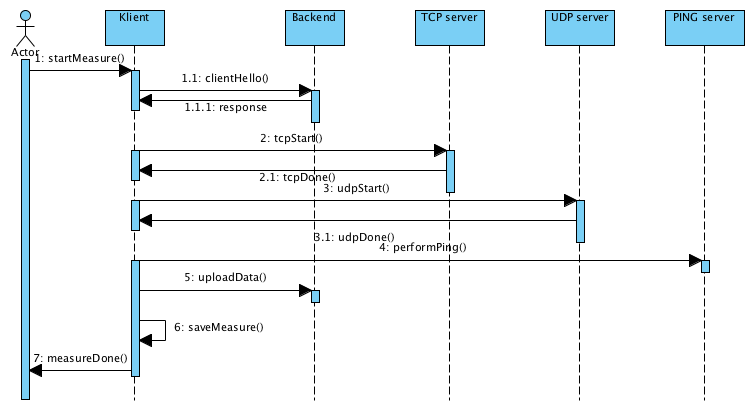
\includegraphics[width=0.8\textwidth]{figures/03_implementation/seq_diagram.jpg}
    \caption{Kompletní průběh měření}
    \label{err1}
\end{figure}

Nakonec proběhne měření odezvy proti PING serveru a spočítání hodnoty jitter. Jitter je změna velikosti zpoždění paketů a počítá se následně \cite{RFC}:

$$ J_i = \frac{J_{i-1} + (|D_{i-1,i}| - J_{i-1})}{16} $$

Výpočet jitteru probíhá iterativně. Hodnota $D_{i-1,i}$ reprezentuje vzdálenost packetů a je ekvivalentní rozdílu relativních přenosových časů. Dělení 16 probíhá pro kvalitní odstranění šumu při zachování přiměřené míry konvergence \cite{JIT}.

Tím měření končí a klient odesílá naměřené údaje na backend.

\section{Běh aplikace na pozadí}
Vyřešit běh na pozadí bylo největším oříškem celé implementace a zároveň klíčovou funkcionalitou, bez které by aplikace byla velice omezená. Základní filosofie společnosti Apple je, jak již bylo zmíněno, že aplikace bude na pozadí provádět jednu z povolených aktivit. Zároveň, jelikož se Apple snaží o to, doručit svým zákazníkům vždy špičkový software, požaduje totéž od vývojářů, a pro účely běhu na pozadí vydal rozhraní pro konkrétní implementaci. V praxi to vypadá tak, že vývojář stanoví v nastavení, že se jedná o aplikaci využívající uživatelovu polohu. Pakliže chce vývojář, aby aplikace běžela na pozadí, využije rozhraní, které odchytává \emph{změny polohy} - nikoliv v čase, nýbrž v prostoru. To bylo ale v rozporu s požadavkem na periodické měření v zadaném intervalu. 

Pokusil jsem se nejprve tuto variantu naimplementovat, tak, že jsem nastavil, aby měl \uv{locationManager}\footnote{Objekt odchytávající údaje o pozici} nejvyšší citlivost. V momentě, kdy tento objekt zachytil změnu, zkontroloval jsem čas a porovnal, jestli už uplynul dostatek od posledního měření. Poté jsem provedl měření. Tato metoda byla při standartním pohybu člověka v průběhu dne relativně přesná, nicméně v noci, kdy telefon leží na stolku, absolutně nefunkční.

Druhý způsob, který se naskytnul, bylo \uv{šťouchnutí} od serveru. Implementace spočívá \\v tom, že aplikace vyžádá ke svému certifikátu tzv. \emph{token}, který se naváže na Apple ID uživatele a zaregistruje se na Apple Push Serverech. Tento token si zároveň uloží server, z kterého bude posílána zpráva do iOS zařízení. Komunikace následně probíhá tak, že server pošle požadavek na Apple Push Server a ten to přepošle do daného iOS zařízení. Tato služba se nazývá APN (Apple Push Notification). Její implementace je elegantní v tom, že zařízení má otevřený jeden socket, přes který může přicházet velké množství zpráv. Nedrží si tak otevřené spojení s každou aplikací, a tím se šetří výdrž baterie. Tuto implementaci jsme ovšem zamítli pro vysokou časovou náročnost jak pro klienta, tak pro serverovou část. Zároveň by byla tato implementace pouze pro klienta iOS, neboť Google má pro svou platformu vlastní službu - GCM (Google Cloud Message) - a ta má zcela odlišnou implementaci.

Třetí způsob, který se nakonec ukázal jako nejefektivnější, se na první pohled zdá jako porušování pravidel Apple. Pokud má aplikace nastaveno, že podporuje běh na pozadí, pak v momentě, kdy ji uživatel minimalizuje, má 10 minut běhu, a pak se sama ukončí. Zjistil jsem, že v těchto deseti minutách stačí alespoň jednou zavolat objekt locationManager a zapnout/vypnout na něm odchytávání pozice uživatele. Tímto se prodlouží životnost probíhané aktivity o dalších 10 minut. Zajistil jsem tedy, že jednou za 9 minut (dal jsem si \\pro jistotu časový polštář) takto zařízení vyžádá pozici a běh na pozadí pokračuje.

\section{Uživatelské rozhraní}
Uživatelské rozhraní je paradoxně to nejdůležitější na celé aplikaci. Funkcionalita je upozaděna, neboť první dojem je zde absolutně klíčový. Jelikož projekt není cílený pouze na profesionály, nýbrž je určený pro širokou veřejnost, není UX\footnote{User experience} okrajovou záležitostí. Uživateli se musí aplikace na první pohled líbit, musí ihned pochopit, k čemu slouží, a zároveň musí aplikace uživateli nabídnout své služby v co nejpřívětivější formě.

Proces návrhu rozhraní podléhal následujícím kritériím:

\begin{enumerate}
	\item Co chceme uživateli prezentovat?
	\item Co všechno opravdu uživatel potřebuje vidět?
\end{enumerate}

\subsection{Pravidla Apple}
Apple si nepřeje, aby UX byla pro každou aplikaci odlišná. Chce, aby uživatelé rozuměli aplikacím hned, protože to poslední, co chce, je, aby o nich někdo říkal, že mají složitá a komplikovaná uživatelská rozhraní. Pro tyto účely vydal pokyny, jak postupovat při procesu návrhu \cite{HIG}.

\subsubsection*{UINavigationController}
Prvním základním stavebním prvkem je Navigation Controller. V hierarchii objektů je postaven nad všemi objekty typu \emph{View}. Zajišťuje přechod obrazovek, a navíc od šesté verze operačního systému iOS odchytává rotaci zařízení.

Jelikož žádný iPhone ani iPad nemají tlačítko zpět, je Navigation Controller obligátním prvkem při postupném zanořování. Uživatelé tedy vědí, že mají hledat tlačítko zpět vždy \\v horním levém rohu.

\subsubsection*{UITableView}
Apple má velice konkrétní představu o tom, jak by měly vypadat tabulky (seznamy). Uživatelé si zvykli na určité typy ikon, které naznačují, co buňka udělá, pokud ji uživatel vybere. Pokud má buňka šipku, uživatel ví, že se po vybrání zanoří hlouběji. Pokud nemá, zůstane na stejné úrovni. 

Velice zajímavý fakt je, že Apple dokázal úspěšně odstranit ze svých uživatelských rozhraní checkboxy pro seznamy. Pokud umožní programátor uživateli provést hromadnou akci s daty, učiní tak přes hromadnou selekci, která se zobrazí po stisku speciálního tlačítka.

\newpage

\subsection{Návrh}
Při navrhování jsem používal prototypovací nástroj Balsamiq, abych si vizualizoval myšlenky a zobrazení dat. Jedná se o jednoduchý WYSIWYG\footnote{What you see is what you get} editor, ve kterém můžeme rychle vytvořit uživatelské rozhraní bez dlouhého programování.

\begin{figure}[h]
	\centering
    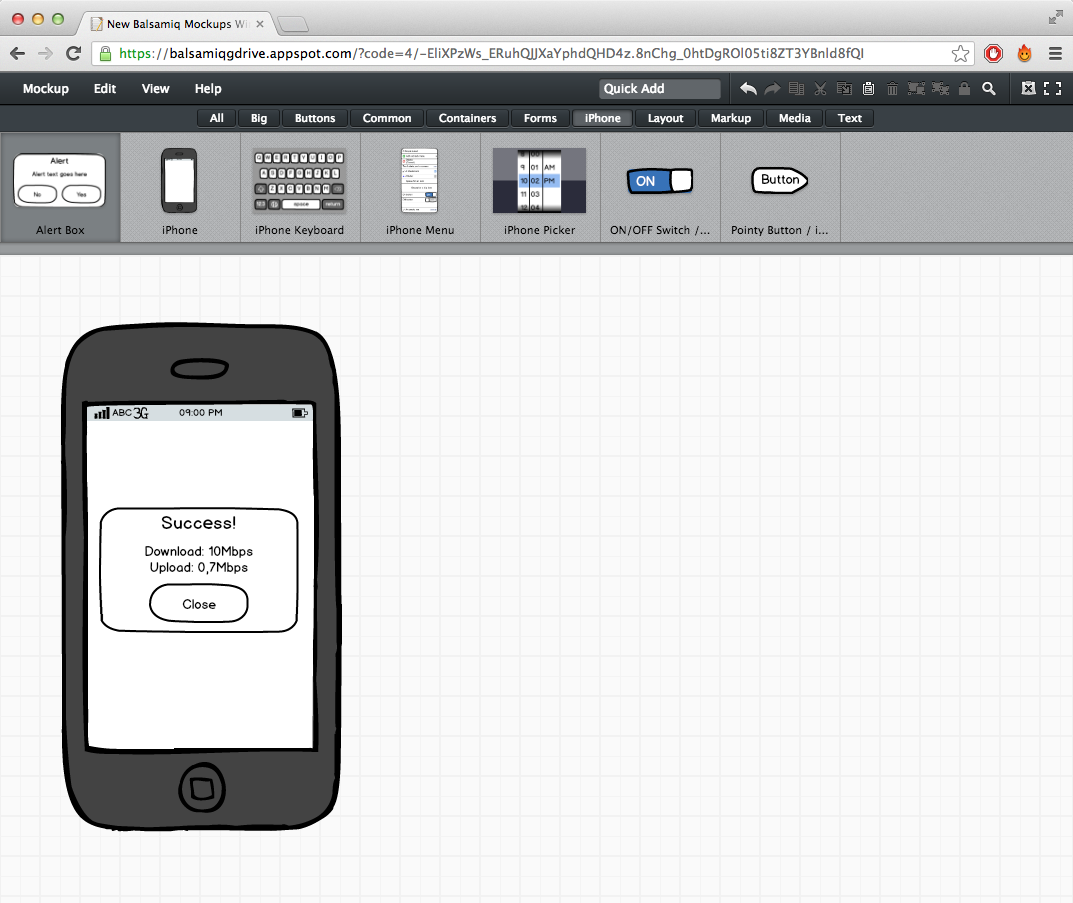
\includegraphics[width=0.8\textwidth]{figures/03_implementation/balsamiq.jpg}
    \caption{Prostředí prototypovacího nástroje Balsamiq v prohlížeči Google Chrome}
    \label{bals}
\end{figure}

\subsection*{Hlavní obrazovka aplikace}

\subsubsection*{Tab bar}
První nápad byl použít tab bar. Je univerzální, je to další ze základních stavebních prvků podle Applu a už jsem ho použil v předchozích aplikacích. Problém s tab barem je, že zůstává neustále na očích, i když ho vlastně uživatel nepotřebuje. 

{\bf Příklad:}
Uživatel začne měřit a sleduje průběh měření. Stěží ho bude zajímat kompletní historie měření. Buď měří jednorázově, tudíž se mu zobrazí výsledek po dokončení měření, nebo měří periodicky a zajímají ho dílčí výsledky provedené v probíhajícím sezení. V tomto případě je spodní bar k ničemu, protože nelze nastavit, aby se choval dvojím způsobem - jeho chování bude vždy konstantní.

Zároveň tab bar určuje jakousi paralelní souběžnost akcí pod jednotlivými záložkami, což je nesmysl, neboť během měření by nemělo být umožněno uživateli měnit nastavení svého účtu. Z toho jsem usoudil, že tab bar není vhodným středobodem rozhraní.

\subsubsection*{Dashboard}
Vrátil jsem se zpět k požadavkům a snažil si uspořádat myšlenky pro nejvhodnější rozložení aplikace. Dospěl jsem k názoru, že dashboard bude optimálním řešením. Nebudu mást uživatele výběrem více obrazovek v tab baru. Po přihlášení dostane na výběr:

\begin{enumerate}
	\item Prohlížet výsledky
	\item Měřit
\end{enumerate}

Pokud si bude chtít prohlédnout dílčí výsledky během měření, podívá se přímo z měření přes speciální tlačítko. Nebude tak muset zkoumat, které výsledky byly v daném měření naměřeny, protože dotaz do databáze se bude vztahovat pouze k danému průběhu.

\subsection*{Zobrazení výsledků}
Výsledky lze zobrazit v seřazeném seznamu podle času měření. Seznam je oddělován delimitery po jednotlivých dnech. Zajímavostí seznamu je, že se dynamicky překreslí, pokud je do databáze zapsáno nové měření. K realizaci takového dynamického seznamu je určeno rozhraní \emph{NSFetchedResultsControllerDelegate} z frameworku Core Data. Pro plnou funkčnost je třeba implementovat čtyři metody:

\begin{enumerate}
	\item
	\emph{- (void)controllerWillChangeContent:(NSFetchedResultsController *)controller}
	
	Zde se musí zavolat metoda \emph{beginUpdates} na objektu \emph{UITableView}, díky kterému se tabulka zamkne a je možné ji bezpečně\footnote{thread safe} začít aktualizovat.
	
	\item
	\emph{- (void)controller:(NSFetchedResultsController *)controller didChangeSection:\\(id <NSFetchedResultsSectionInfo>)sectionInfo atIndex:(NSUInteger)sectionIndex \\forChangeType:(NSFetchedResultsChangeType)type}
	
	Tato metoda se stará o konzistenci jednotlivých sekcí. Jak je zmíněno výše, sekce jsou děleny po jednotlivých dnech.
	
	\item
	\emph{- (void)controller:(NSFetchedResultsController *)controller didChangeObject:\\(id)anObject atIndexPath:(NSIndexPath *)indexPath forChangeType:\\(NSFetchedResultsChangeType)type newIndexPath:(NSIndexPath *)newIndexPath}
	
	Tato metoda je k dispozici pro odlišení, zda byl objekt z databáze smazán, nebo byl nový objekt přidán. Slouží pro identifikaci nové akce a zapracování animace.

	\item
	\emph{- (void)controllerDidChangeContent:(NSFetchedResultsController *)controller}
	
	Pokud je tato metoda zavolána, znamená to, že veškeré úpravy byly dokončeny. Programátor by v této metodě měl uvolnit paměť, kterou použil při aktualizaci tabulky, a nakonec by ji měl odemknout. Tím proces končí.
\end{enumerate}

\subsection{Grafické zpracování}
Pro zpracování grafického vzhledu rozhraní jsem použil Adobe Photoshop CS 5.5. V průběhu implementace jsem našel v designu zalíbení, nicméně časová náročnost byla velmi vysoká, protože jsem neznal prostředí Photoshopu, a celý týden jsem se snažil zorientovat ve všech funkcionalitách.

\subsubsection*{Barvy a logo}
Během diskuzí s celým týmem došlo ke sjednocenému názoru, že aplikace by měla být laděná do tónů modré barvy. Osobně preferuji realistické barvy nad pastelové, rozhodl jsem se tedy podtrhnout barvy světlem a logo jsem vytvořil stříbrné. Obě zmíněné konkurenční aplikace mají v logu tachometr, proto jsem tvorbu loga odlišil. Nebyl jsem si jistý, co použít a chtěl jsem se vyhnout klišé tachometru. Prozatím zůstává tedy logem stříbrný nápis MBTest \\s použitým písmem Agency FB. Výsledné logo a postup jeho přípravy se nachází v příloze.

\subsubsection*{Rozměry obrazovek}
Do vydání páté generace iPhone měl Apple velice chytře vyřešenou otázku rozlišení. Všechny modely do verze 3GS měly stejné displaye. První verze s displayem \emph{retina}, iPhone 4, předchozí rozlišení zdvojnásobil, tudíž byly zachované poměry stran. V praxi to fungovalo následovně:

Jedno tlačítko má rozměr 30 x 80 na nižším rozlišení a 60 x 160 na vyšším. Projekt tedy musí obsahovat dva PNG soubory - btn\_img.png a btn\_img@2x.png. Klíčové rozšíření je \uv{@2x}, které dává kompilátoru pokyn pro výběr tohoto souboru pro vytvoření GUI pro iPhone s vyšším rozlišením.

\begin{table}[h]
	\begin{center}
		\begin{tabular}{|l|l|}
			\hline
				{\bf Model} & {\bf Rozlišení}\\
			\hline \hline
				iPhone & 320 x 480\\
				\hline
				iPhone 3G & 320 x 480\\
				\hline
				iPhone 3GS & 320 x 480\\
				\hline
				iPhone 4 & 640 x 960\\
				\hline
				iPhone 4S & 640 x 960\\
				\hline
				iPhone 5 & 640 x 1136\\
				\hline
		\end{tabular}
	\end{center}
	\caption{Tabulka rozlišení jednotlivých modelů iPhone}
	\label{tab.resphone}
\end{table}

Jak je patrné z tabulky, model iPhone 5 má odlišný poměr stran od ostatních modelů a vyladění drobných detailů v grafickém rozhraní se musí řešit v kódu, čímž kód poněkud klesá na kvalitě a přenosnosti.

\newpage
Tablety iPad jsou v tomto ohledu jednotné a veškeré modely si zachovaly stejný poměr stran.

\begin{table}[h]
	\begin{center}
		\begin{tabular}{|l|l|}
			\hline
				{\bf Model} & {\bf Rozlišení}\\
			\hline \hline
				iPad & 1024 x 768\\
				\hline
				iPad 2 & 1024 x 768\\
				\hline
				iPad 3 & 2048 x 1536\\
				\hline
				iPad 4 & 2048 x 1536\\
				\hline
				iPad mini & 1024 x 768\\
				\hline
		\end{tabular}
	\end{center}
	\caption{Tabulka rozlišení jednotlivých modelů iPad}
	\label{tab.restab}
\end{table}

Nasazení grafiky u iPadu pro vyšší rozlišení funguje stejně jako u iPhone. Na konferenci společnosti Apple - WWDC 2013 mají být odhaleny nové verze obou stávajících modelů tabletu iPad, nicméně indície vedou ke stejnému rozlišení u obou verzí (2048 x 1536).

\chapter{Testování}

\section{Uživatelské testy}
Cílem uživatelských testů bylo zjistit, zda mnou zvolené rozhraní bylo správné řešení. Důležitá je totiž intuitivnost rozhraní pro uživatele, aby s ním dokázal pracovat rychle a efektivně.

\subsection{Příprava na test}
Jelikož je certifikace cizích zařízení složitá, zvolil jsem jako testovací přístroj vlastní iPhone, který jsem testovaným osobám dával s připravenou ikonou na obrazovce ke spuštění.

\subsection{Průběh testu}

\subsubsection*{1. kolo}

\begin{enumerate}
	\item Spustit aplikaci
	\item Vstoupit do aplikace jako anonymní uživatel
	\item Změřit jednorázově
	\item Změřit kvalitu sítě
	\item Zobrazit naměřené hodnoty
\end{enumerate}

\subsubsection*{2. kolo}

\begin{enumerate}
	\item Spustit aplikaci
	\item Vstoupit do aplikace jako uživatel se jménem \emph{test} a heslem \emph{test}
	\item Nastavit periodické měření pro každých 30 vteřin
	\item Pustit měření kvality sítě
	\item Minimalizovat aplikaci
	\item Vyčkat 2 minuty
	\item Vrátit se do aplikace a podívat se na doposud naměřené hodnoty
	\item Přerušit měření
\end{enumerate}

\subsection{Vyhodnocení testu}

\begin{table}[h]
	\begin{center}
		\begin{tabular}{|c|c|c|}
			\hline
				{\bf Krok} & {\bf Osoba A} & {\bf Osoba B}\\
			\hline \hline
				1. & OK & OK\\
				\hline
				2. & OK & OK\\
				\hline
				3. & OK & OK\\
				\hline
				4. & OK & OK\\
				\hline
				5. & OK & OK\\
				\hline \hline
				1. & OK & OK\\
				\hline
				2. & OK & OK\\
				\hline
				3. & OK & OK\\
				\hline
				4. & OK & OK\\
				\hline
				5. & OK & OK\\
				\hline
				6. & OK & OK\\
				\hline
				7. & OK & OK\\
				\hline
				8. & OK & OK\\
				\hline
		\end{tabular}
	\end{center}
	\caption{Tabulka úspěšnosti uživatelských testů}
	\label{tab.usr}
\end{table}

Všem dotázaným bylo předem řečeno, že nebude možné odpovídat na jejich dotazy. Osoba B se v případě nastavení periodického měření ptala na překlad, ale nakonec se to obešlo bez komplikací.

\subsubsection{Závěr}
Aplikace byla vyhodnocená jako intuitivní a přehledná. Tyto výstupy hodnotím pozitivně a je to jasný signál, že jde uživatelské rozhraní tou správnou cestou.

\newpage

\section{Funkční testy}

\subsection{Prostředky pro testování}
Součástí SDK pro iOS je simulátor iOS zařízení. Narozdíl od \emph{emulátoru} DVM v SDK \\pro Android, iOS simulátor nepřepočítává procesorové funkce a spouští se velmi rychle. Běh aplikace je simulován věrohodně a rychlost je velmi blízká reálnému zařízení. Pro rozsáhlé testování je ovšem nevhodný, protože neodráží skutečný svět. Neříká nic o výdrži baterie, a zároveň má stálé, pevné připojení k internetu.

Pro účely testování jsem měl mimo simulátor k dispozici zařízení:

\begin{enumerate}
	\item iPhone 5
	\begin{itemize}
		\item O2-CZ
		\item Neomezený datový tarif
		\item iOS 6.1.4 (10B350)
	\end{itemize}
	
	\item iPad 2
	\begin{itemize}
		\item O2-CZ
		\item 10GB FUP
		\item iOS 5.1.1 (9B206)
	\end{itemize}
\end{enumerate}

\begin{figure}[htp]
	\centering
	\label{figur}

  	\subfloat[iPhone 5] {
  		\label{figur:1}
  		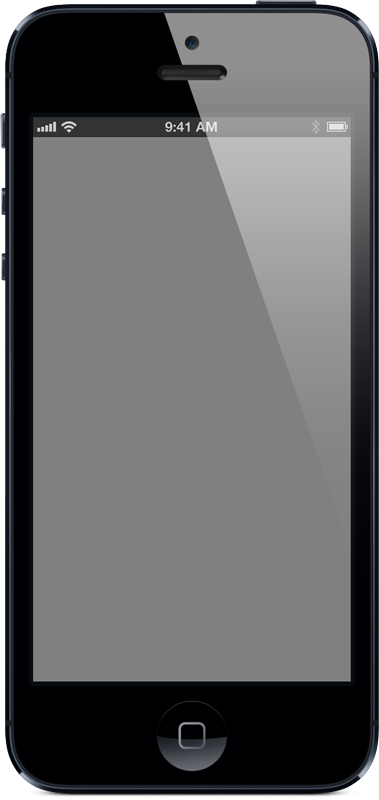
\includegraphics[width=0.18\textwidth]{figures/04_testing/iphone.jpg}
  	}
  		\qquad
  	\subfloat[iPad 2] { 
  		\label{figur:2}
  		
\includegraphics[width=0.3\textwidth]{figures/04_testing/ipad.jpg}
  	}
	\caption{Zařízení k testování} (nejedná se o reálný poměr velikostí)
\end{figure}

\newpage

\subsection{Výdrž baterie}

\subsubsection{Příprava na test}
Pro účely testování výdrže baterie v telefonu jsem využil iPhone 5. Nahrál jsem do něj aktuální verzi aplikace a plně jsem jej nabil. Telefon byl během testu používán v každodenních činnostech - telefonování, psaní sms, elektronická pošta, focení a prohlížení webových stránek.

\subsubsection{Průběh testu}

\subsubsection*{1. kolo}

\begin{enumerate}
	\item Spustit aplikaci
	\item Přihlásit se pod vlastním účtem
	\item Spustit periodické měření na každých 30 vteřin
	\item Minimalizovat aplikaci
	\item Pravidelně kontrolovat, zda aplikace nespadla
	\item Sledovat stav baterie do 5\% nabití
\end{enumerate}

\subsubsection*{2. kolo}

\begin{enumerate}
	\item Spustit aplikaci
	\item Přihlásit se pod vlastním účtem
	\item Spustit periodické měření na každých 15 minut
	\item Minimalizovat aplikaci
	\item Pravidelně kontrolovat, zda aplikace nespadla
	\item Sledovat stav baterie do 5\% nabití
\end{enumerate}

\newpage

\subsubsection{Vyhodnocení testu}
V nepravidelných intervalech jsem kontroloval stav baterie a zaznamenával jej do tabulky v obou kolech. V používání telefonu jsem se nelimitoval.

\subsubsection*{1. kolo}

\begin{table}[h]
	\begin{center}
		\begin{tabular}{|l|c|}
			\hline
				{\bf Čas} & {\bf Stav nabití baterie}\\
			\hline \hline
				13:50 & 98\%\\
				\hline
				14:10 & 97\%\\
				\hline
				14:25 & 95\%\\
				\hline
				14:35 & 93\%\\
				\hline
				14:40 & 91\%\\
				\hline
				14:45 & 90\%\\
				\hline
				15:05 & 85\%\\
				\hline
				15:15 & 82\%\\
				\hline
				15:25 & 78\%\\
				\hline
				15:45 & 72\%\\
				\hline
				15:55 & 70\%\\
				\hline
				16:15 & 65\%\\
				\hline
				16:25 & 62\%\\
				\hline
				16:40 & 59\%\\
				\hline
				16:45 & 58\%\\
				\hline
				17:00 & 55\%\\
				\hline
				17:15 & 51\%\\
				\hline
				17:35 & 46\%\\
				\hline
				17:55 & 42\%\\
				\hline
				18:20 & 35\%\\
				\hline
				18:50 & 28\%\\
				\hline
				19:15 & 23\%\\
				\hline
				19:50 & 16\%\\
				\hline
				19:50 & 9\%\\
				\hline
				20:30 & 5\%\\
				\hline
		\end{tabular}
	\end{center}
	\caption{Tabulka naměřených hodnot stavu nabití baterie - 1. kolo}
	\label{tab.30s}
\end{table}

Telefon se za velice krátkou dobu vybil (necelých 7 hodin). Při intervalu 30 vteřin provedl měření celkem 827krát (nenechal jsem ho měřit do úplného vybití).

\newpage

\begin{figure}[h]
	\centering
	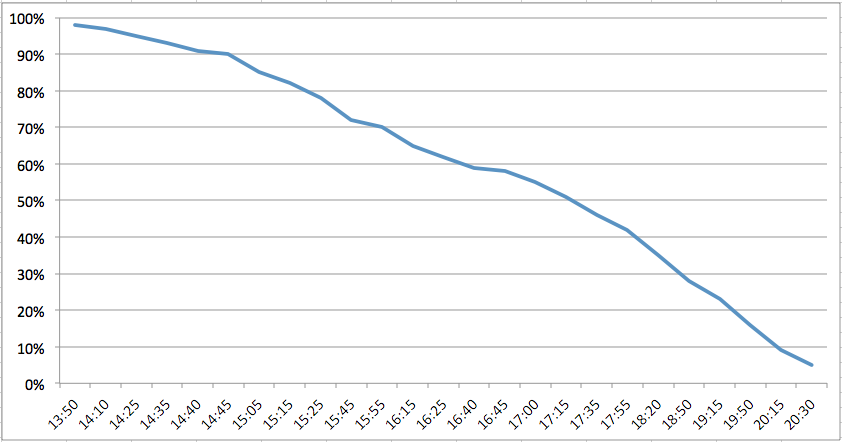
\includegraphics[width=0.8\textwidth]{figures/04_testing/graph30.jpg}
	\caption{Stav baterie vzhledem k času při měření s intervalem 30 vteřin}
	\label{batt1}
\end{figure}

\subsubsection*{2. kolo}
\begin{table}[h]
	\begin{center}
		\begin{tabular}{|l|c|}
			\hline
				{\bf Čas} & {\bf Stav nabití baterie}\\
			\hline \hline
				9:00 & 99\%\\
				\hline
				10:00 & 94\%\\
				\hline
				11:00 & 87\%\\
				\hline
				12:00 & 83\%\\
				\hline
				13:00 & 77\%\\
				\hline
				14:00 & 75\%\\
				\hline
				15:00 & 71\%\\
				\hline
				16:00 & 66\%\\
				\hline
				17:00 & 63\%\\
				\hline
				18:00 & 57\%\\
				\hline
				19:00 & 51\%\\
				\hline
				20:00 & 46\%\\
				\hline
				21:00 & 41\%\\
				\hline
				22:00 & 38\%\\
				\hline
		\end{tabular}
	\end{center}
	\caption{Tabulka naměřených hodnot stavu nabití baterie - 2. kolo}
	\label{tab.15m}
\end{table}

Telefon změřil kvalitu sítě při intervalu 15 minut  92krát. Ve 22:00 měl stále dostatečně nabitou baterii pro standartní používání (38\%).

\newpage

\begin{figure}[h]
  	\centering
    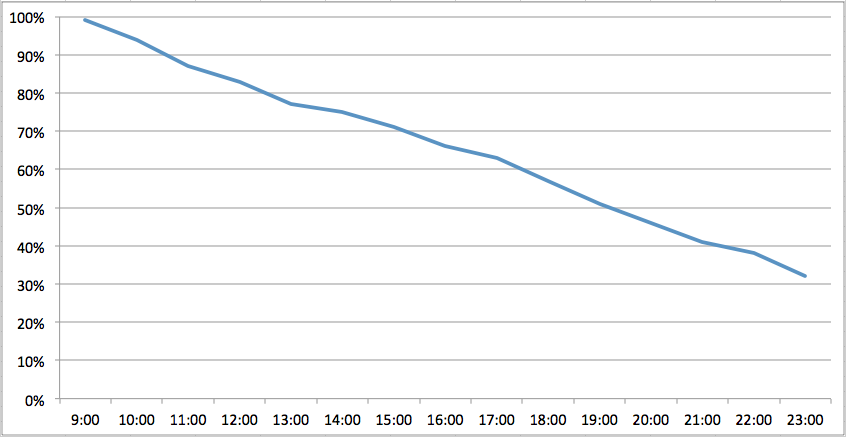
\includegraphics[width=0.8\textwidth]{figures/04_testing/graph15.jpg}
    \caption{Stav baterie vzhledem k času při měření s intervalem 15 minut}
    \label{batt2}
\end{figure}

\subsubsection*{Závěr}
Testy vyhodnocuji pozitivně. Pro měření s velice krátkým intervalem vydrží telefon měřit kvalitu sítě 7 hodin při standartním používání. Pokud bude chtít uživatel měřit s větším intervalem, rozdíl ve výdrži baterie téměř nepozná.

\subsection{Test kvality měření oproti konkurenci}

\subsubsection{Příprava na test}
Pro testování kvality měření oproti konkurenčním aplikacím jsem použil iPhone 5 s nainstalovanými aplikacemi DSL.cz, Speedtest.net a MBTest. Telefon měl v průběhu měření vypnutou WiFi a byl v okruhu dobrého připojení do sítě 3G (FEL ČVUT, Karlovo Náměstí).

\subsubsection{Průběh testu}

\begin{table}[h]
	\begin{center}
		\begin{tabular}{|l|c|}
			\hline
				{\bf Aplikace} & {\bf Naměřená rychlost download/upload}\\
			\hline \hline
				Speedtest.net & 5.61 Mbps/1.16 Mbps\\
				\hline
				DSL.cz & 4.19 Mbps/1.53 Mbps\\
				\hline
				MBTest & 4.70 Mbps/1.26 Mbps\\
				\hline
		\end{tabular}
	\end{center}
	\caption{Tabulka naměřených hodnot měřících aplikací}
	\label{tab.speed}
\end{table}

\subsubsection*{Vyhodnocení testu}
Zpočátku se vyskytly potíže nepřesného měření. Řešením bylo nastavení větší velikosti bufferu na socketu na straně klienta. Výstupy hodnotím kladně a považuji drobné odchylky za zanedbatelné.

\chapter{Závěr}

\section{Splněné cíle práce}
Jelikož bylo v projektu MBTest zainteresováno více lidí, přirozeně přicházely často nové podněty a nápady pro funkcionalitu. Některé byly zapracovány, některé ne. Základní požadavky však byly beze zbytku splněny a celý systém lze prohlásit za funkční.

Mně osobně nejvíce bavila implementační část. Musel jsem se vypořádat se zákazy Applu a najít korektní cesty, jak vyřešit danou problematiku (například běh na pozadí). Zároveň jsem se naučil implementovat TCP/UDP komunikaci v jazyce Objective-C a objevil jsem nástupce ASIHTTPRequest frameworku - AFNetworking framework, kterého hodlám hojně používat v dalších projektech.

\section{Budoucí funkce}
Bohužel nebylo možné implementovat veškeré vysněné funkce, které vznikly během společných konzultací a sezení celého týmu. Největší překážku, kterou jsem musel překonat, byl běh na pozadí, který mě zaměstnal téměř na dva měsíce vývoje. Takové zdržení mi nedovolilo implementovat tyto funkcionality:

\begin{enumerate}
\item Graficky propracované GUI

Rád bych zapracoval kompletní grafické zpracování s vlastními navrženými komponentami.
\item Pokročilá animace průběhu měření

Aplikace by měla být líbivá, neboť vzhled je u dnešních aplikací na prvním místě. Zároveň screenshoty v App Store jsou první náhled do aplikace pro uživatele - podle nich se rozhoduje, zda ji stáhne, nebo ne.
\item Pokročilá detekce chyb při měření

Rád bych vytvořil \uv{chytřejší} odchytávání chyb. Automat by se učil a sám rozhodoval, proč chyba nastala a co může dělat, aniž by přerušil měření a prohlásil jej za neúspěšné.
\item Lokální push notifikace o vykonaném měření

Pro uživatele by bylo jistě zajímavé, kdyby mohl mít zpětnou vazbu o průběhu měření na pozadí ve formě push notifikací.
\item Zobrazení jednotlivých i více výsledků na mapě

Velice zajímavá funkce je zobrazení mapy průběhu měření - odkud kam uživatel šel. \\K tomu je potřeba v pravidelných intervalech ukládat pozici zařízení.
\item Zobrazení grafu rychlostí v daném časovém úseku

Statistiky jsou vždy zajímavé i na menším displayi. Pro uživatele by bylo jistě přínosné je  přehledně zobrazit v grafu.
\end{enumerate}

\section{Budoucnost projektu}
Projekt nevnímám jako ukončený. Rád bych jej vylepšoval a přidával nové funkcionality. Vidím prostor pro zlepšování prezentace dat uživateli. Zařízení s iOS mají již v této době poměrně výkonný hardware a jistě by se dal využít k složitějším statistickým výpočtům. Jelikož jsem spojil svou budoucnost s programem OI, nevidím důvod, proč bych neměl na projektu nadále pokračovat.

%*****************************************************************************

\bibliographystyle{misc/csplainnat}
\bibliography{reference}

%*****************************************************************************

\appendix

\chapter{Seznam použitých zkratek}

\begin{description}
\item[ARC] Automatic Reference Counting
\item[TCP] Transmission Control Protocol
\item[UDP] User Datagram Protocol
\item[PING] Packet InterNet Groper
\item[SDK] Software Development Kit
\item[API] Application Programming Interface
\item[DVM] Dalvik Virtual Machine
\item[FUP] Fair User Policy
\item[REST] Representational State Transfer
\item[UX] User experience
\item[QA] Quality Assurance
\item[BTS] Base Transceiver Station
\item[WYSIWYG] What You See Is What You Get
\end{description}
\vdots
\chapter{Grafický návrh}
\section{Přihlašovací obrazovka}
První, co uživatel uvidí, rozhodne o tom, zda si aplikaci nechá. Může se to jevit až vágní, nicméně první dojem hraje velice důležitou roli. Proto jsem zvolil realistický, jednoduchý design.

\begin{figure}[h]
	\begin{center}
		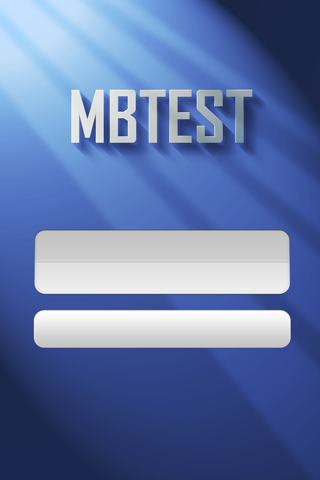
\includegraphics[width=5cm]{figures/AX_graphics/login_screen.jpg}
		\caption{Přihlašovací obrazovka pro iPhone 5}
		\label{fig:login}
	\end{center}
\end{figure}

V návrhu nejsou obsažené texty, ty se doplňují kvůli lokalizaci až v Xcode. Horní dvě kolonky jsou vstupy pro \emph{uživatelské jméno} a \emph{heslo}. Tlačítko má jednu zajímavost. Pokud jsou kolonky prázdné, nese nápis \uv{Anonymous}. Po stisknutí nabídne uživateli dialog, zda chce do aplikace opravdu vstoupit jako anonymní uživatel, nebo jestli nechce přejít raději na stránky a zaregistrovat se. Pokud jsou ovšem obě dvě kolonky vyplněné, nápis se změní na \uv{Sign in}. Tímto krokem jsem chtěl zamezit vzniku dalšího tlačítka, které by rozbilo kompaktní design obrazovky.

\subsubsection*{Proces tvorby}
Nejprve se musí stanovit, odkud světlo půjde. Zvolil jsem metodu \uv{západ slunce}, tudíž jsem umístil zdroj světla do levého horního rohu. 
Dále bylo nutné uvědomit si pořadí vrstev, protože na tom stojí celý vzhled. Pro každou komponentu vypíchnu nejdůležitější kroky.

\begin{enumerate}
	\item {\bf Text}
	\begin{enumerate}
		\item Po vytvoření nápisu bylo třeba text rozkopírovat zhruba desetkrát šikmo dolu s černou maskou. Na tuto vrstu jsem posléze použil funkci \emph{Motion Blur}.
		\item Pro vystoupení hran textu jsem nad textem vytvořil novou vrstu vyplněnou bílou barvou. Vrstvu jsem označil, posunul o pixel šikmo dolu a celou smazal. Tím zůstaly bílé obrysy po levé straně textu tvořící prostorový vjem.
	\end{enumerate}
	\item {\bf Světlo}
	\begin{enumerate}
		\item Nejprve jsem přes text vytvořil různě široké obdelníky, které jsem posléze vyrotoval po směru světla a upravil, aby z rohu vycházely. Nastavil jsem jim 20\% Opacity a použil funkci \emph{Gaussian Blur}.
		\item Nejproblematičtější, ale zároveň nejdůležitější krok, je synchronizace světla a stínu s textem. Na to bylo potřeba vytvořit novou masku paprsků s označením textu, čímž se vytvořil stín přesně tam, kde měl.
		\item Poslední, již kosmetická úprava, bylo oživení světla pomocí filtru \emph{Lightning Effects}. Použil jsem nastavení \emph{Spotlight}, a to dodalu světlu život.
	\end{enumerate}
\end{enumerate}
\chapter{Instalační a uživatelská příručka}

\section{Instalace z App Store}

\begin{enumerate}
	\item Otevřít App Store v zařízení iPhone nebo iPad
	\item Zadat do vyhledávání \uv{MBTest}
	\item Zmáčknout tlačítko stáhnout (aplikace je zdarma)
	\item Vyčkat na stáhnutí a instalaci (aplikace je menší než 50MB - je možné ji stáhnout bez WiFi\cite{APPIN})
\end{enumerate}

\section{Vlastní kompilace zdrojových souborů}

\begin{enumerate}
	\item Otevřít MBTester.xcodeproj v Xcode IDE verzi 4.2.5 a vyšší
	\item V záložce Build Settings, kolonka Code Signing, je třeba podepsat kód vlastním certifikátem
	\item Připojit zařízení s aktivním vývojářským účtem
	\item Zmáčknout tlačítko \emph{Build \& Run}
\end{enumerate}

\section{Jak aplikaci používat}

\subsection{Uživatel}
Po spuštění aplikace uvítá uživatele přihlašovací obrazovka. Uživatel se může buď přihlásit, nebo pokračovat anonymně. Pokud uživatel nevyplní jméno a heslo, bude dotázán, zda chce opravdu pokračovat anonymně, nebo zda si chce vytvořit účet - v tomto případě bude přesměrován na webové stránky, aby se zaregistroval. Neregistrovaný uživatel má uložené pouze lokálně naměřená data v telefonu, a nemůže tak prohlížet své výsledky včetně statistik na webu projektu.

Pro odhlášení stačí na hlavní obrazovce zmáčknout tlačítko v levém horním rohu v navigační liště.

\subsection{Měření}
Měření je možné spustit zmáčknutím tlačítka \emph{Measure} na hlavní stránce aplikace. Následující obrazovka nabídne uživateli zvolení parametrů měření - velikost souboru pro upload a download, zda chce měřit periodicky, potažmo při jaké periodě.
Během měření může uživatel aplikaci minimalizovat, ale ne vypnout.

\subsection{Výsledky}
Dílčí výsledky lze prohlížet přímo z obrazovky probíhajícího měření. Stačí zmáčknout tlačítko \uv{Results} v horním pravém rohu v navigační liště.

Pro zobrazení kompletní historie naměřených výsledků daného zařízení je třeba přejít na hlavní obrazovku (pokud probíhá měření, bude přerušeno). Na hlavní obrazovce je třeba zmáčknout tlačítko \emph{History}. Tím přejde uživatel do seznamu všech měření.
\chapter{Obsah přiloženého CD}
\begin{verbatim}
/CD
|-- ios_app             - zkompilovaná aplikace
|-- ios_src    
|   |-- mbtester        - zdrojové kódy k měřící aplikaci
|   |-- doc             - dokumentace ke zdrojovým kódům           
|-- thesis
|   |-- pdf             - bakalářská práce v PDF formátu
|   |-- latex           - zdrojové kódy textu bakalářské práce
\end{verbatim}

%*****************************************************************************

\end{document}